
\lstinputlisting[language=bash,basicstyle=\small]{python_codes/fieldstone_109/keywords}

\begin{center}
Code at \url{https://github.com/cedrict/fieldstone/tree/master/python_codes/fieldstone_109}
\end{center}

\par\noindent\rule{\textwidth}{0.4pt}

%%%%%%%%%%%%%%%%%%%%%%%%%%%%%%%%%%%%%%%%%%%%%%%%%%%%%%%%%%%%%%%%%%%%%%%%%%%%%%%%%%%%%%%%%%%%%%%%%%%%


This stone reproduces the lower crust experiment explained in \stone~108 coming from 
Clark \etal (2005) \cite{clbr05}.

The domain is $1000\times500\times15~\si{\km}$. Gravity is set to zero so density is irrelevant. 
Boundary conditions are no slip at the top and bottom, free slip on $y=0$ and $y=L_y$ and 
a parabolic Poiseuille flow is prescribed on $x=0$ and $x=L_x$:
\[
u(z)=U_0 \frac{4z(L_z-z)  }{L_z^2}
\]
with $U_0=80~\si{\mm\per\year}$.

The obstacle is centered on $(L_x/2,0)$ and has a radius of $a=200~\si{\km}$ (because of the symmetry of the problem
I only model half of the domain).
It is assigned a viscosity $\eta=2\cdot 10^{21}~\si{\pascal\second}$ which is 1000 times larger than the viscosity
of the channel $\eta=2\cdot 10^{18}~\si{\pascal\second}$.

\begin{center}
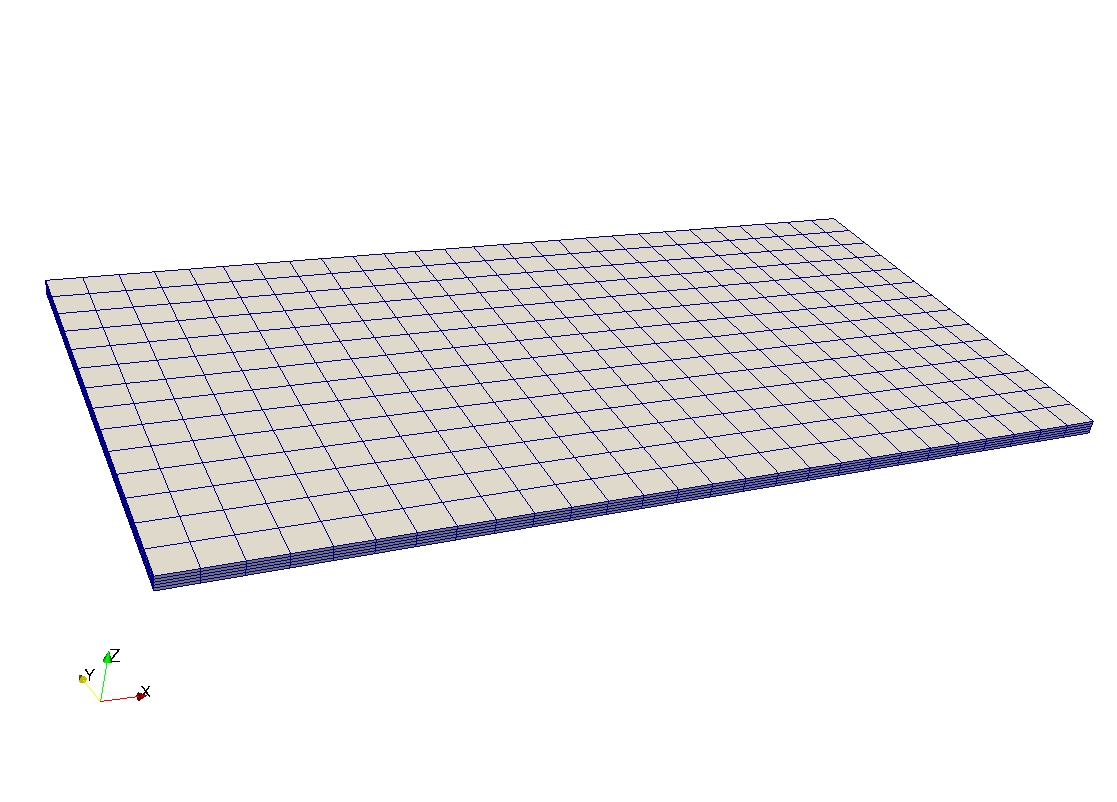
\includegraphics[width=7cm]{python_codes/fieldstone_109/images/grid}
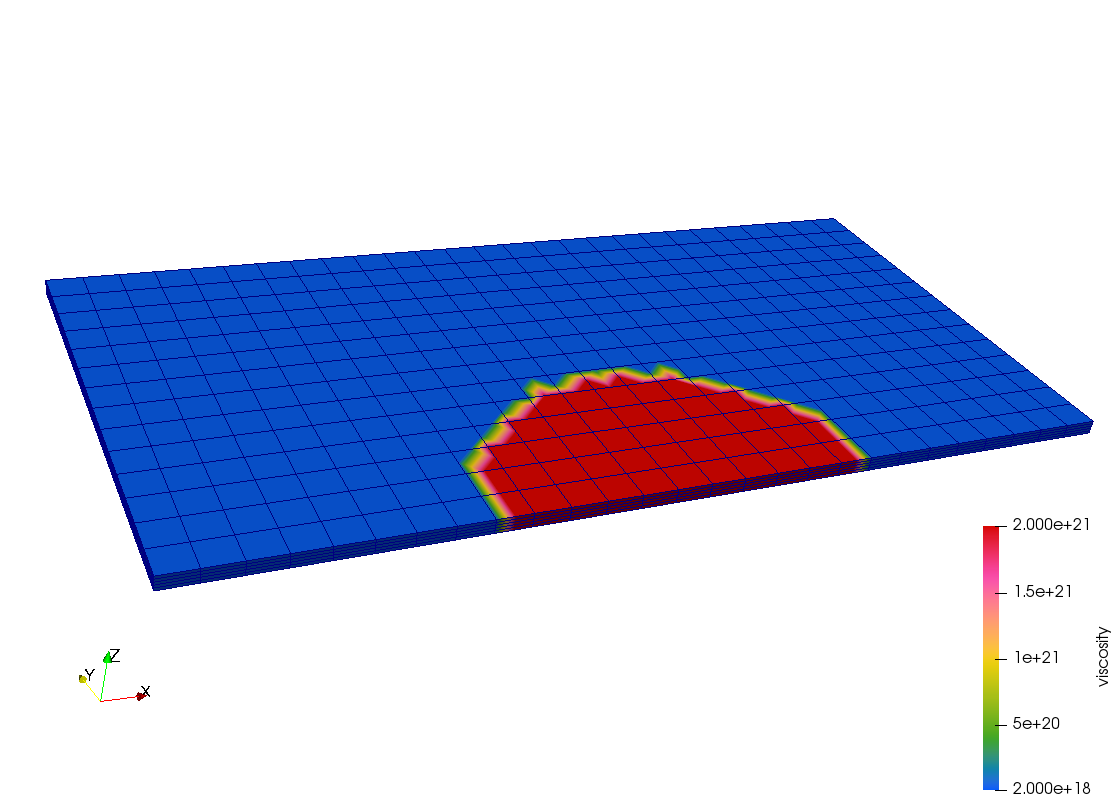
\includegraphics[width=7cm]{python_codes/fieldstone_109/images/eta}
\end{center}

Given the boundary conditions there is a pressure nullspace which is 
removed by enforcing that pressure is volume normalised, i.e. $\int_\Omega p \; dV=0$. The element used is the 
Taylor-Hood pair $Q_2\times Q_1$ (see Section~\ref{ss:pairq2q1}).
The numbering of the nodes follows the one of the VTK format as shown hereunder. 
In retrospect it is not the most straightforward one but it is irrelevant with regards 
to the calculations. A complete layout of the nodes is present in the images folder of this stone. 

\begin{center}
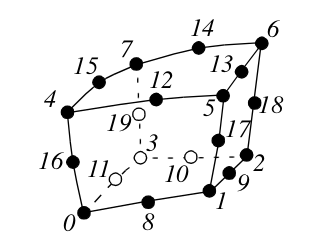
\includegraphics[width=5.5cm]{python_codes/fieldstone_109/images/numbering}
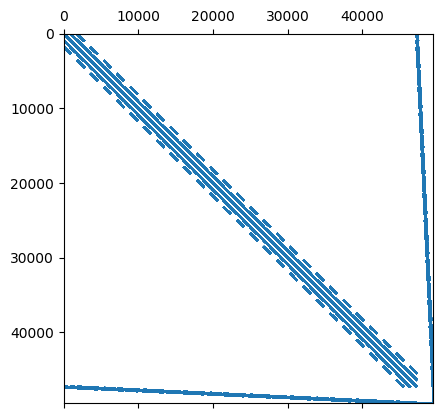
\includegraphics[width=5cm]{python_codes/fieldstone_109/images/matrix}\\
{\captionfont Left: Node numbering of the 20 first nodes; Right: matrix structure}
\end{center}

Because of the direct solver the resolution is rather limited and the maximum is 
about $27\times 14 \times 5$ (the solver then claims about 26+ Gb). The analytical pressure  
\[
p(r,\theta) = 
-\frac{1}{\kappa} U r  \cos \theta
 -\frac{U a^2 }{\kappa r}  \cos \theta
\]
is also computed and projected onto the mesh (pressure is then set to zero inside the 
obstacle) (where $U=2U_0/3$, see \stone 108). 

%------------------------------
\subsubsection*{Benchmarking}

By setting the viscosity of the obstacle to the same value as the rest 
of the domain the problem becomes a classical Poiseuille flow problem, as 
described in Section~\ref{ss:poiseuille}.
In this case the pressure gradient $\Pi$ is related to the velocity profile 
as follows:
\[
u(z) = \frac{1}{2}\frac{\Pi}{\eta_0} (z^2 - zH)
\]
with $\Pi=\frac{\partial p}{\partial x}<0$, i.e. 
there is more pressure applied to the left than to the right of the channel.

Looking above at our applied boundary velocity we find that 
\[
\frac{1}{2}\frac{|\Pi|}{\eta_0} = \frac{4U_0}{L_z^2}
\]
or, $|\Pi|\simeq 18.03$. The domain is 1000~\si{\km} long 
so $\Delta P = |\Pi| L_x \simeq 18,027,001$ i.e. we expect the pressure to 
be $90,135,005~\si{\pascal}$ at $x=0$ and $-90,135,005~\si{\pascal}$ at $x=L_x$. 

\begin{center}
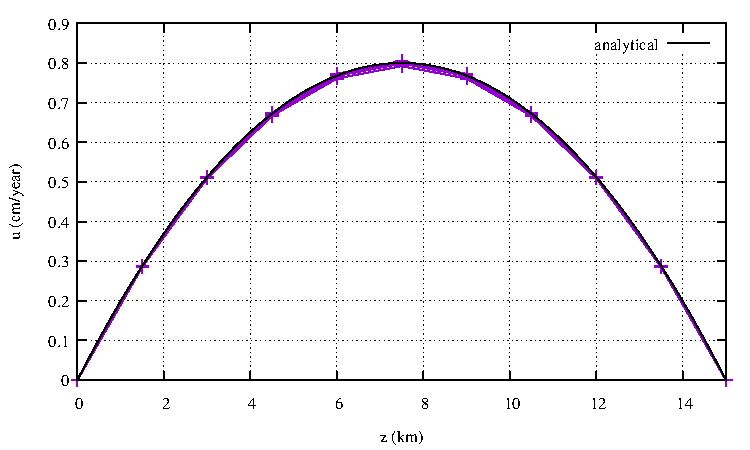
\includegraphics[width=7cm]{python_codes/fieldstone_109/results/bench/vel}
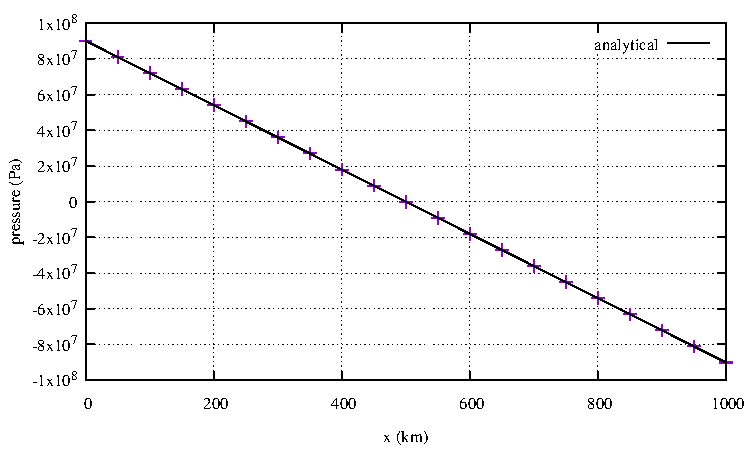
\includegraphics[width=7cm]{python_codes/fieldstone_109/results/bench/press}\\
{\captionfont Computed velocity and pressure fields for the whole domain.}
\end{center}

The computed velocity and pressure fields match their analytical counterparts 
so we can now turn to the problem at hand.

%------------------------------
\subsubsection*{Application}

We find that the computed pressure is rather similar to the analytical pressure, although 
amplitudes differ by about 20\%. This is likely due to the finite size of the domain while 
the analytical solution assumes an infinite domain around the obstacle.

\begin{center}
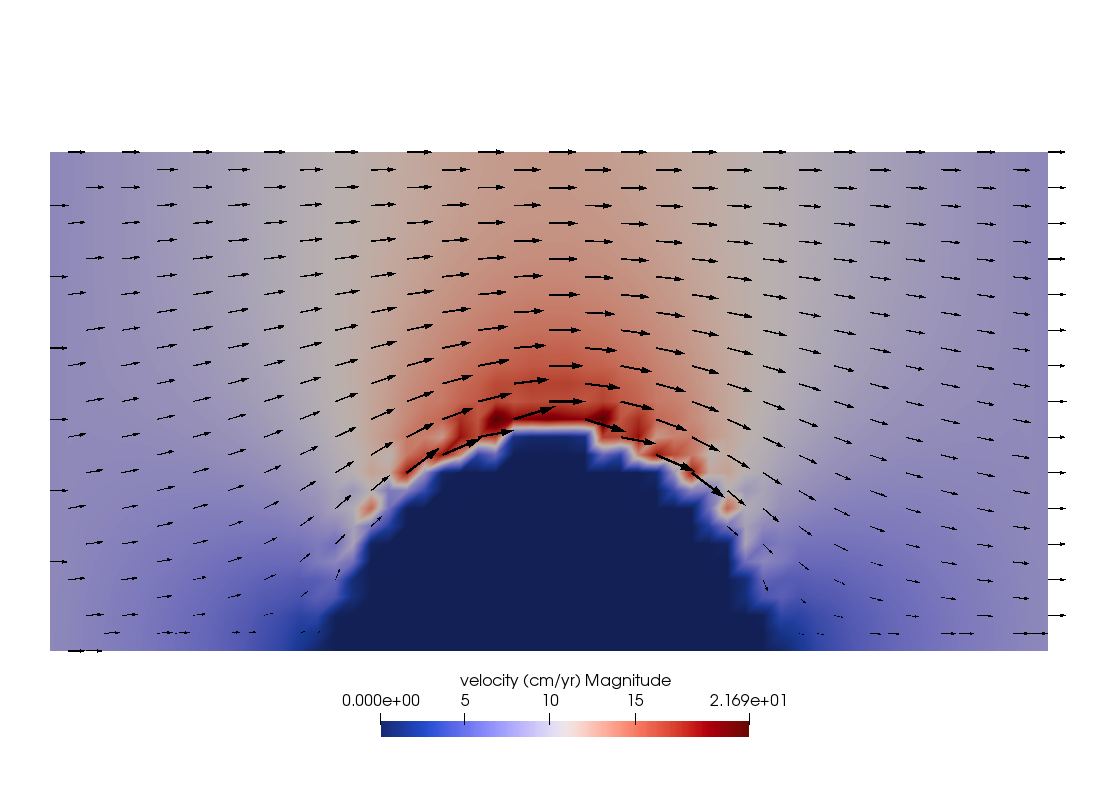
\includegraphics[width=5.4cm]{python_codes/fieldstone_109/results/vel}
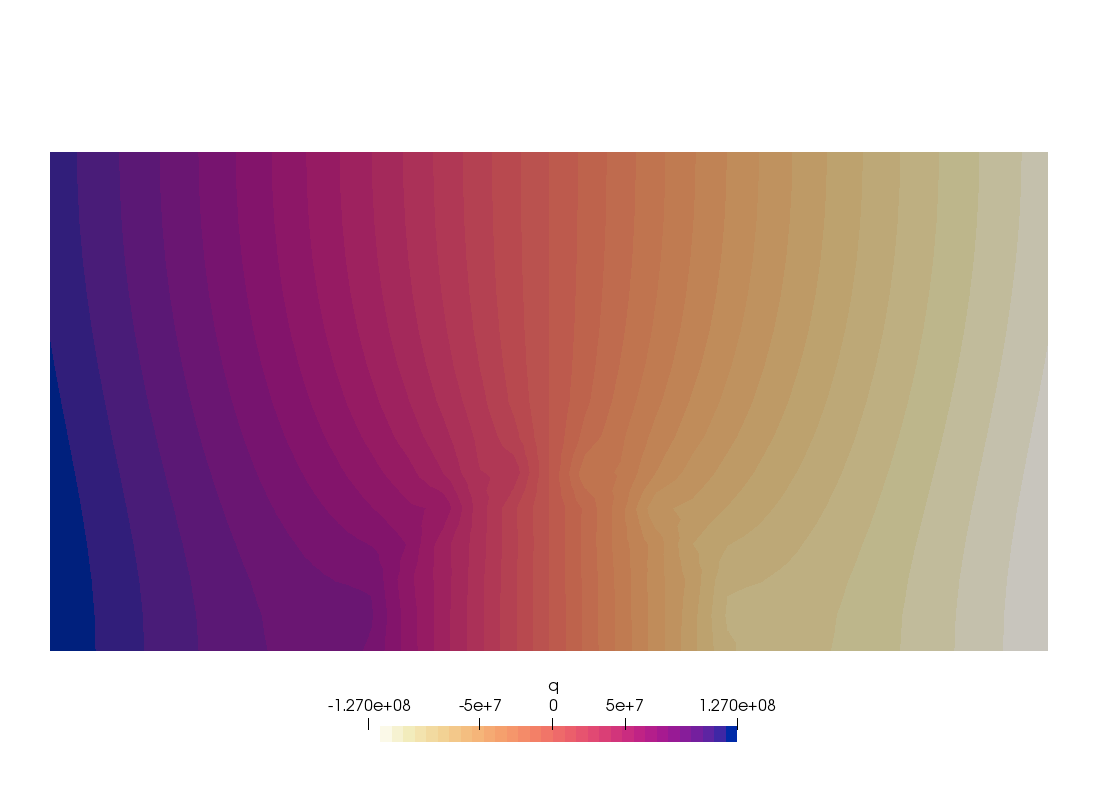
\includegraphics[width=5.4cm]{python_codes/fieldstone_109/results/press}
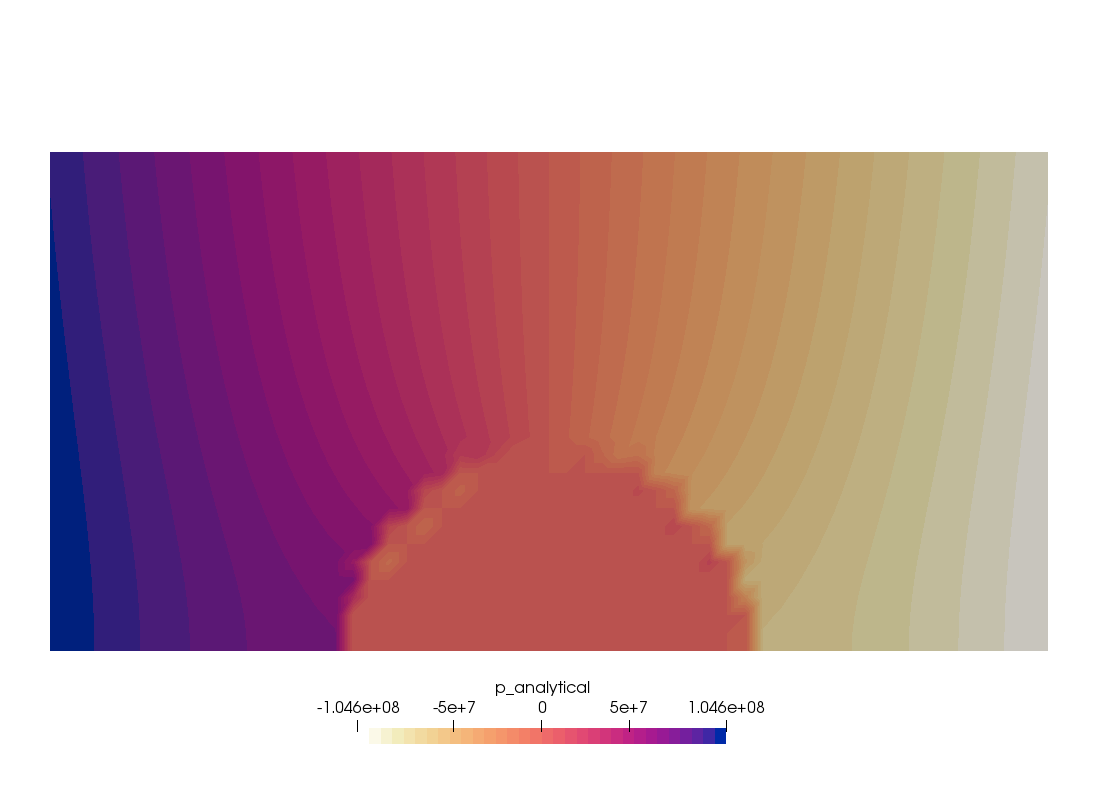
\includegraphics[width=5.4cm]{python_codes/fieldstone_109/results/press_anal}\\
{\captionfont Velocity, pressure and analytical pressure fields. }
\end{center}

Note that the computed pressure does not depend on the $z$-coordinate (while of course the velocity does): 
\begin{center}
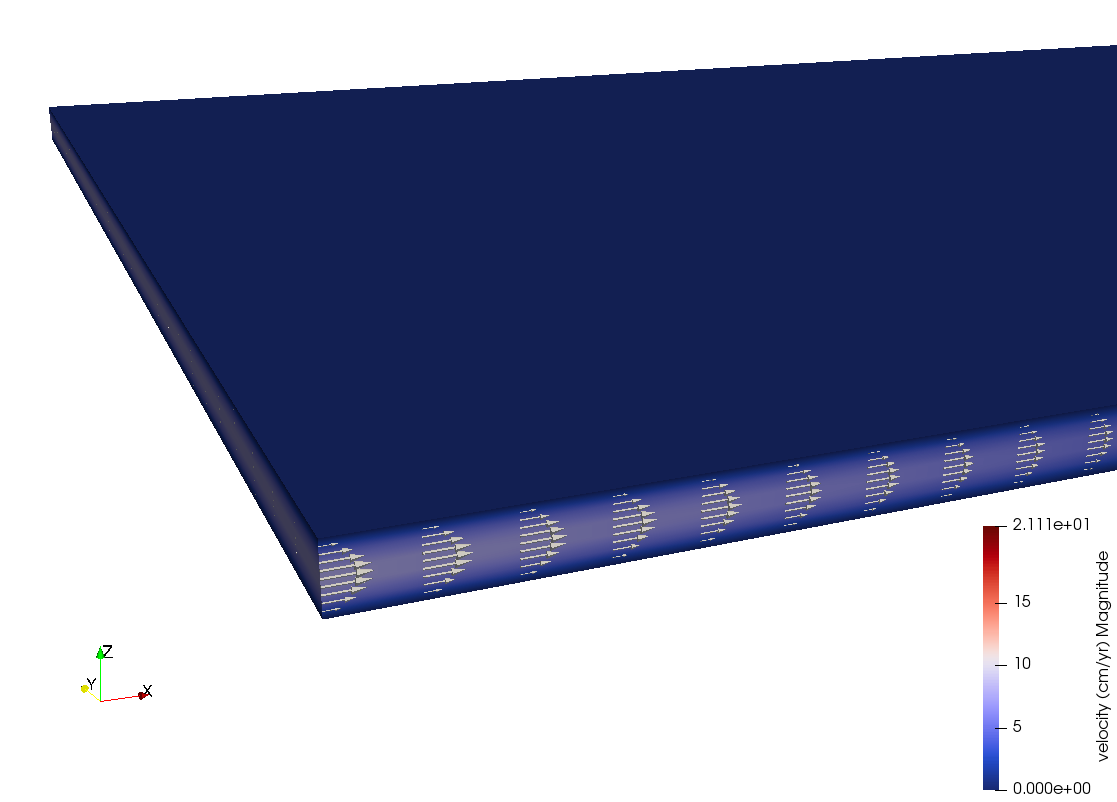
\includegraphics[width=5.4cm]{python_codes/fieldstone_109/results/vel2}
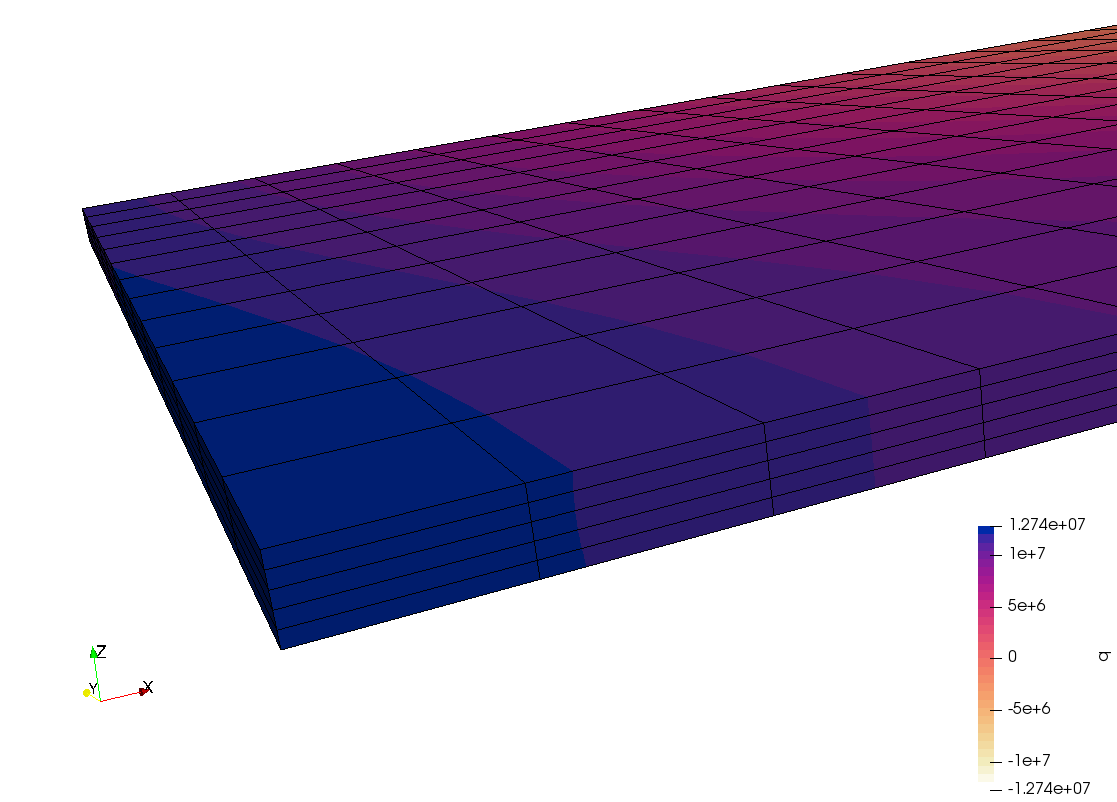
\includegraphics[width=5.4cm]{python_codes/fieldstone_109/results/press2}\\
{\captionfont Velocity and pressure fields. We see that the aspect ratio of the elements
is rather large and this is likely to alter the accuracy of the calculations.}
\end{center}

The recovered pressure is rather similar to the analytical one. Indeed we find that an increase in resolution and 
an increase in domain size (especially $L_z$) brings the computed pressure closer and closer to the 
analytical one. At the max resolution that fits on my 32Gb laptop pressures are off by less than 10\%.

I have also run this experiment with the \aspect code and the prm file is present in 
the folder of this stone. Resolution was higher than above ($160 \times 80 \times 16 =204,800$ elements).

\begin{center}
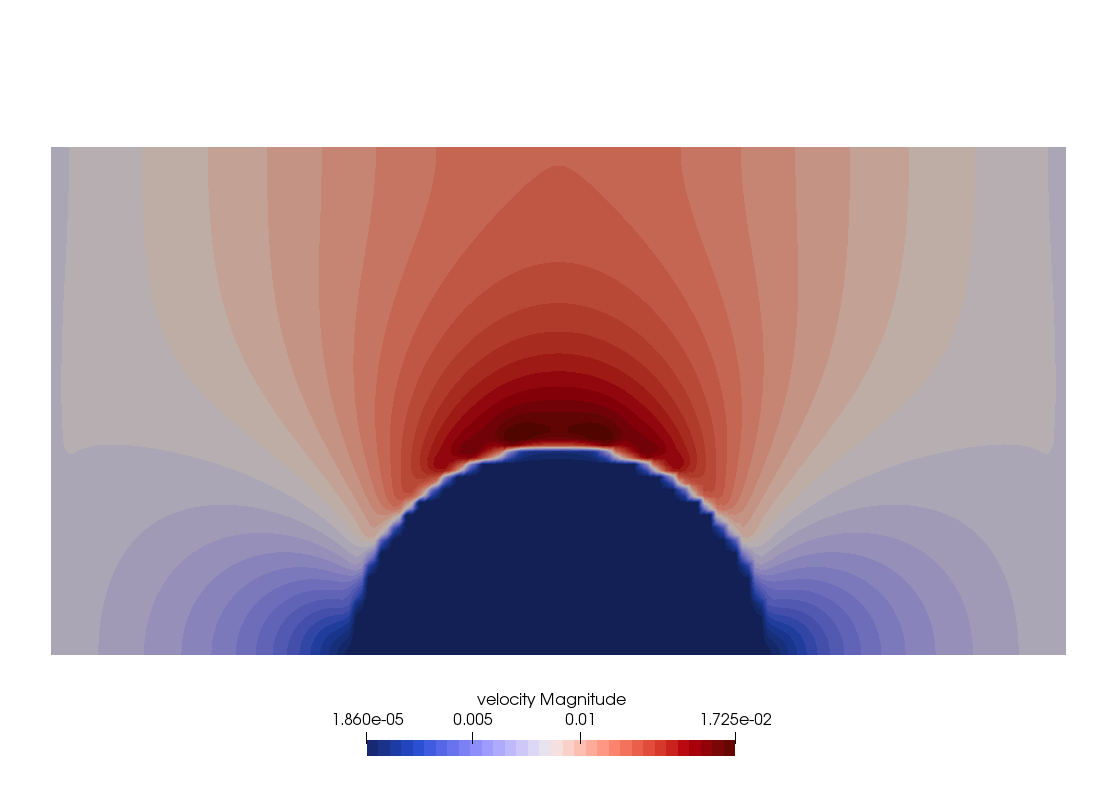
\includegraphics[width=7cm]{python_codes/fieldstone_109/results/aspect/vel}
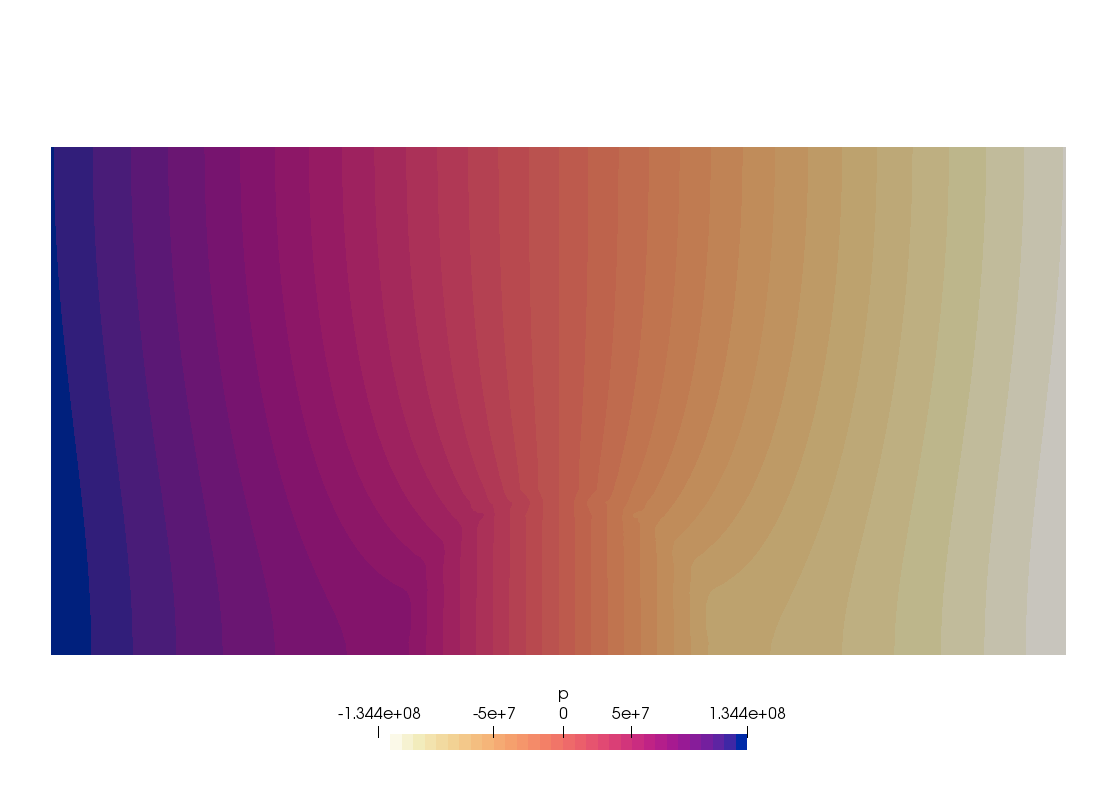
\includegraphics[width=7cm]{python_codes/fieldstone_109/results/aspect/press}\\
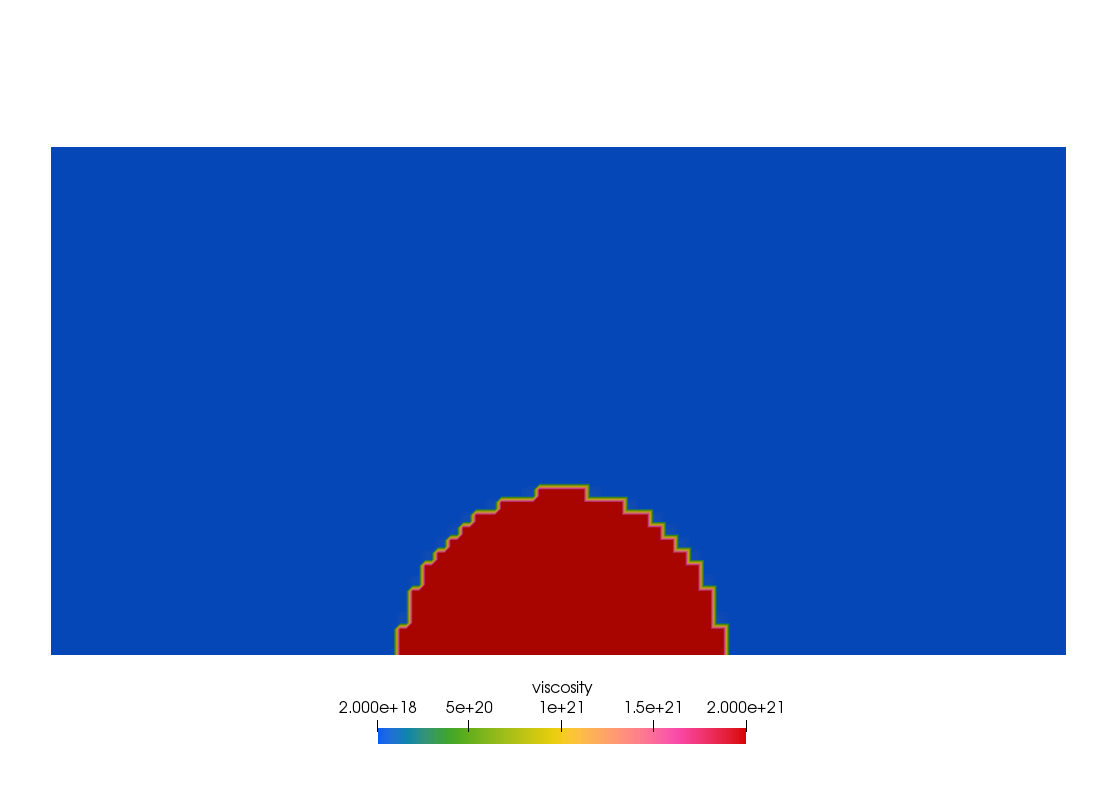
\includegraphics[width=7cm]{python_codes/fieldstone_109/results/aspect/eta}
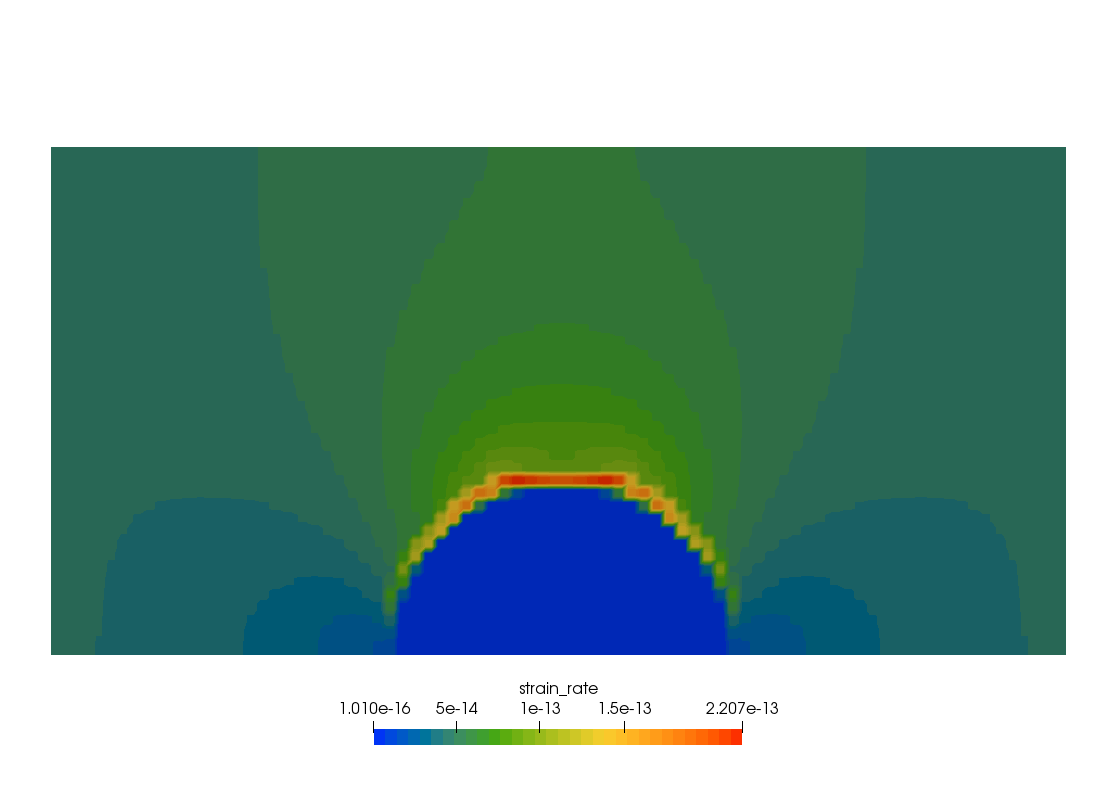
\includegraphics[width=7cm]{python_codes/fieldstone_109/results/aspect/sr}
\end{center}

We find that the results obtained with \aspect do not differ substantially from those
obtained with this stone, despite a much higher resolution.

We find that the pressure min and max are quite larger than the isoviscous case (about 12.35MPa instead 
of 9.014MPa).  



